\chapter{Project development: web application for \\ multimedia editing}
\label{ch:ch3_ProjectDevelopment}

% --- Chapter 3 start ---

This chapter concludes  the main thesis about remix culture by combining most of the topics presented in the previous chapters into a practical example of project development. Namely, the results of the final project and the perspective taken on the software development process cover  topics such as: remix as a cultural phenomenon, considerations about contents legal liability and the associated rights, accompanied  by organisational considerations when working for and within an interdisciplinary context and project environment\footfullcite{CleanCode}\footfullcite{EloquentJavascript}.

\section{Reusability and maintainability, through abstractions to a component based approach}

Modern software development techniques and tendencies are mainly concerned with the objective of simplifying the development of technical solutions, as well as easing up code reusability and maintainability.

\section{Web Components}

Web components are a set of Web APIs that allow to create custom, reusable HTML elements with logic and styling encapsulated into their definition. From a practical point of view, modern browsers can compute Web Components in the form of custom HTML tags that, in turn, can be used and re-used across multiple projects and technology stacks. The described behaviour is equivalent to the one of standard HTML elements as defined in the HTML documentation.

\subsection{JavaScript Modules}

JavaScript modules (also known as “ES Modules” or “ECMAScript Modules”) are core to the modern web development and can be considered as a prerequisite for the Web Components technology. The definition of a module seems to be quite consistent across the subject literature. A module can be defined as: “… a piece of program that specifies which other pieces it relies on and which functionality it provides for other modules to use (its interface).”

\subsection{Custom Elements}

Custom Elements, as defined in the W3C living standard.

\subsection{Shadow DOM}

Shadow DOM API as referred in W3C living standard.

\subsection{HTML Templates}

The HTML Templates technology consists of HTML template.

\section{Web Components libraries}

Web Components libraries were created with the main intent of simplifying and speeding up the development process. Libraries usually provide some sort of abstractions on top of the native Web Components for efficiency and in order to enable new features.

\section{Project idea and Front End Software Architecture}

In this section, a brief discussion about the project idea and its evolution will be introduced followed by a description of the adopted front end software architecture.

\begin{figure}[H]
\centering
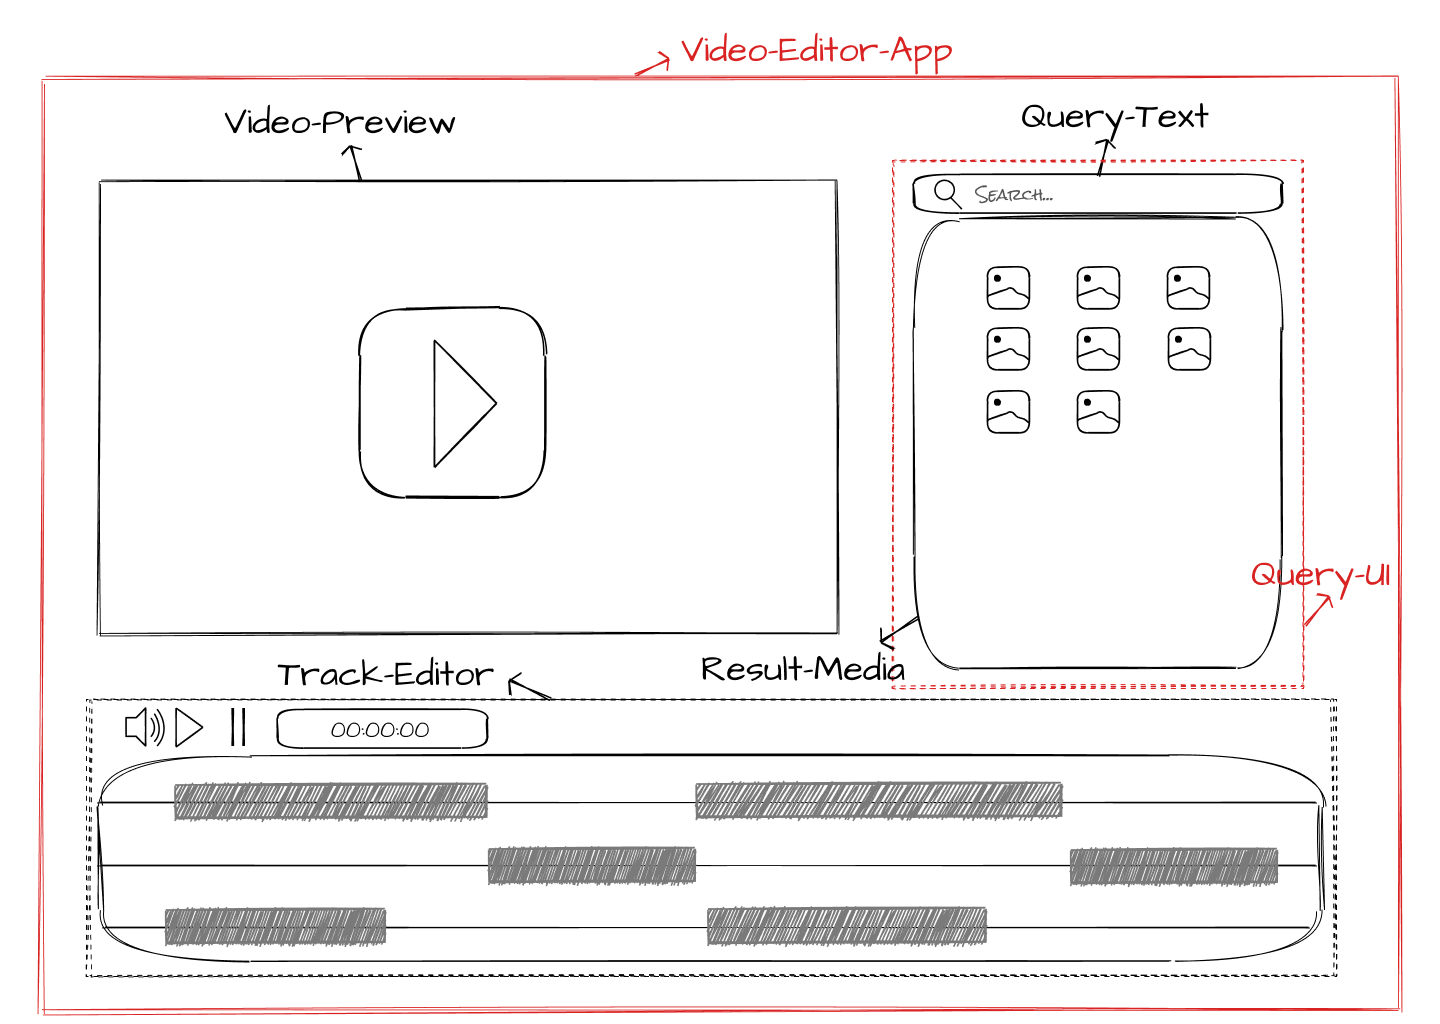
\includegraphics[width=1\textwidth]{images/Wireframe.png}
\caption{Application Mock-up}
\label{fig:appMockUp}
\end{figure}


\section{Searching and displaying results}

Searching and displaying the retrieved results can be considered pivotal for applications whose success can be largely measured in terms of the quantity and the quality of offered resources.

\subsection{Search component}

The Search component, named “Query-Text”.

\subsection{Results viewer component}

As the name suggests, the “Media-Result” component renders some results onto the interface.

\section{Multimedia Editor}

The most characterizing piece of this project is the Multimedia Editor.

\subsection{Track Editor component}

“Track-Editor”.

\subsection{Media Preview component}

The final part of this application is the media preview. 

\section{Application examples}

To be continued.

\subsection{PH-Remix}

To be continued.

\subsection{Multimedia Editor}

To be continued.